% 
%
% (c) 2025 Autor, ETH Zürich
%
% !TEX root = linalg_I-II_summary.tex
% !TEX encoding = UTF-8
%

\section{Dual Spaces \& Inner Products}
Let $V$ be a vector space over $K$ (any field). Recall that we have the dual space $V^{\ast} := \operatorname{Hom}(V, K) =$ the space of linear maps $\varphi :V \to K$ (functionals). $V^{\ast}$ is also a vector space over $K$.

Consider now an inner product space $(V, \langle \cdot , \cdot \rangle)$ over $K = \mathbb{R}$ or $\mathbb{C}$. Let $u \in V$. Define
\[
	\varphi_u :V \to K, \quad V \owns v \mapsto \langle v, u \rangle \in K.
\]
$\varphi_u$ is linear since, $v$ is the first argument in the scalar/hermitian product.

\begin{theorem}{Canonical 'Almost' Isomorphism between $V$ and $V^{\ast}$}{can_iso_dual_sp}
	Let $(V, \langle \cdot, \cdot \rangle)$ be a finite dimensional inner product space over $K = \mathbb{R}$ or $\mathbb{C}$. Let $\varphi \in V^{\ast}$. Then there exists a \textbf{unique} $u \in V$ s.t. $\varphi = \varphi_u$, i.e., $\varphi(v) = \varphi_u(v) \quad \forall \, v \in V$.
	
	In fact, for $K = \mathbb{R}$ the map $\Phi:V \to V^{\ast}$, given by $\Phi(u):= \varphi_u$ is an isomorphism.
	
	For $K = \mathbb{C}$, this map is injective and surjective but only $\mathbb{C}$-anti linear, i.e.,
	\begin{align*}
		\Phi(u_1 + u_2) &= \Phi(u_1) + \Phi(u_2) \qquad \forall \,  u_1, u_2 \in V\\
		\Phi(c u) &= \overline{c} \cdot \Phi(u) \qquad \forall \, c \in \mathbb{C}, u \in V.
	\end{align*}
\end{theorem}
So, at least for $K = \mathbb{R}$, a scalar product on $V$ gives us a canonical isomorphism $V \cong V^{\ast}$. (But this isomorphism depends on the scalar product!)

\subsection{\textcolor{red}{The Adjoint Map}}
\label{sec:adj_map}
(Everything in this Subsection should be learned by heart.)
Let $V, W$ be vector spaces over $K$. Let $T:V \to W$ be a linear map. We have seen in Subsection \ref{sec:dual_map} that $T$ induces a linear map (the dual map) 
\[
	T^{\ast}:W^* \to V^*, \quad T^*(\varphi) := \varphi \circ T.
\]

Assume now that $(V, \langle \cdot , \cdot \rangle_V)$ and $(W, \langle \cdot , \cdot \rangle_W)$ are inner product spaces over $K = \mathbb{R}$ or $\mathbb{C}$. Assume also that \underline{$\dim V < \infty$}. Given $T$ as above, we can define $T' :W \to V$ using our 'canonical' identifications $W \cong W^*$, $V \cong V^*$. (No problem for $K = \mathbb{R}$, but we have to be careful with $K = \mathbb{C}$.)

\begin{figure}[H]
	\centering
	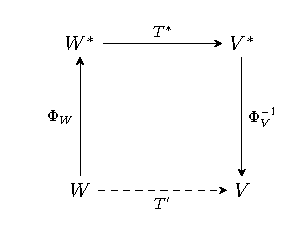
\includegraphics[scale=1.2]{doc/adjoint_map/adjoint_map.pdf}
\end{figure}
i.e. $T' := \Phi_V^{-1} \circ T^* \circ \Phi_W$. We've also used that $\dim V < \infty$, b.c. then $\Phi_V$ is bijective.

What properties does $T'$ have? Note that $T'$ is uniquely determined by
\begin{align*}
	\Phi_V \circ T' = T^* \circ \Phi_W \quad &\Longleftrightarrow \quad \forall w \in W : \; \Phi_V \circ T'(w) = T^*\circ \Phi_W(w)\\
	&\Longleftrightarrow \quad \varphi_{T'(w)} = T^* \circ \varphi_w \; (\in V^*)\\
	&\Longleftrightarrow \quad \forall v \in V : \; \varphi_{T'(w)}(v) = \big(T^*\circ \varphi_w\big)(v)\\
	&\Longleftrightarrow \quad \langle v, T'(w) \rangle_V = \varphi_w\big(T(v)\big) = \langle T(v), w \rangle_W.
\end{align*}
In other words,
\[
	\langle Tv, w \rangle_W = \langle v, T'w \rangle_V \qquad \forall \, v \in V, w \in W.
\]

\textbf{Claim:} $T'$ is a linear map.

\begin{proof}
	For $K = \mathbb{R}$, $\Phi_W, \Phi_V$ and $T^*$ are linear. Therefore, $T'$ is linear too.
	
	For $K = \mathbb{C}$, $\Phi_W, \Phi_V$ are additive but only $\mathbb{C}$-anti linear. Therefore, $\Phi_V^{-1}$ is also additive and $\mathbb{C}$-anti linear. Indeed, let $y_1, y_2 \in V^*$. Since $\Phi_V$ is bijective, we can find unique $x_1, x_2 \in V$ s.t. $\Phi_V(x_1) = y_1$ and $\Phi_V(x_2) = y_2$. Since $\Phi_V$ is additive we have that
	\[
		\Phi_V^{-1}(y_1 + y_2) = \Phi_V^{-1}\big(\Phi_V(x_1) + \Phi_V(x_2)\big) = \Phi_V^{-1}\big(\Phi_V(x_1 + x_2)\big) = x_1 + x_2 = \Phi_V^{-1}(y_1) + \Phi_V^{-1}(y_2).
	\]
	Similarly, let $c \in \mathbb{C}, y \in V^*$. We again can find a unique $x \in V$ s.t. $\Phi_V(x) = y$. Since $\Phi_V$ is $\mathbb{C}$-anti linear we have that
	\[
		\Phi_V^{-1}(cy) = \Phi_V^{-1}\big(c \cdot \Phi_V(x)\big) = \Phi_V^{-1}\big(\Phi_V(\overline{c}x)\big) = \overline{c} \cdot x = \overline{c} \cdot \Phi_V^{-1}(y).
	\]
	So, we have shown that $\Phi_V^{-1}$ is additive and $\mathbb{C}$-anti linear as well.
	
	Now, we return to the proof of the claim. We recall that $T^*$ is linear. Let $w_1, w_2 \in W$ be arbitrary. Since $T^*$ is in particular additive and $T' = \Phi_V^{-1} \circ T^* \circ \Phi_W$, we can conclude that $T'$ is also additive.
	Now, let $c \in \mathbb{C}, w \in W$. Since $T^*$ is linear and $\Phi_V^{-1}, \Phi_W$ are $\mathbb{C}$-anti linear we have that
	\begin{align*}
		T'(cw) &= \Phi_V^{-1} \circ T^* \circ \Phi_W(cw) = \Phi_V^{-1}\Big(T^*\big(\overline{c}\cdot \Phi_W(w)\big)\Big) = \Phi_V^{-1}\Big(\overline{c}\cdot T^*\big(\Phi_W(w)\big)\Big)\\
		&= c \cdot \Phi_V^{-1}\Big(T^*\big(\Phi_W(w)\big)\Big) = c \cdot T'(w).
	\end{align*}
	This proves the claim. \qedhere
\end{proof}

\textbf{Notation:} The linear map $T' :W \to V$ is denoted many times by $T^*:W \to V$. This makes sense b.c. of the 'canonical' identifications. But we have to assume additionally that $ \dim W < \infty$. The map $T^*:W \to V$ is called the \textbf{adjoint} of $T$.

\subsection{Basic Properties of Adjoint Maps}
\begin{lemma}{\textcolor{red}{Properties of Adjoint Maps}}{prop_adj_map}
	Let $V, W, U$ be finite dimensional inner product spaces over $K = \mathbb{R}$ or $\mathbb{C}$. Let $S, T:V \to W$ and $R:W \to U$ be linear maps. Then:
	\begin{enumerate}
		\item $T^*$ is a linear map.
		\item $(S + T)^* = S^* + T^*$.
		\item $\forall \lambda \in K : \; (\lambda T)^* = \overline{\lambda}T^*$.
		\item $(T^*)^* = T$.
		\item $(id_V)^* = id_V$.
		\item $(R \circ T)^* = T^* \circ R^*$.
	\end{enumerate}
\end{lemma}

\begin{proof}
	Let $y_1, y_2 \in V$. We'll repeatedly use that if $ \forall \, x  \in V:\;\langle x, y_1\rangle = \langle x, y_2\rangle$, then $y_1 = y_2$. This is because 
	\begin{align*}
		\forall \, x \in V :\;\langle x, y_1\rangle = \langle x, y_2\rangle \qquad &\Longrightarrow \qquad \forall x \in V :\; \langle x, y_1 - y_2\rangle = 0\\
		\Longrightarrow \qquad y_1 - y_2 = 0 \qquad &\Longrightarrow \qquad y_1 = y_2,
	\end{align*}
	where we've used 2. of Lemma \ref{lem*prop_euclid_sp}
	
	\textbf{1)} Has already been proven in Subsection \ref{sec:adj_map}.
	
	\textbf{2)} Let $w \in W, v \in V$. By the defining properties of $T^*, S^*$ we have that
	\begin{align*}
		\langle v, (S + T)^*w \rangle = \langle (S + T)v, w \rangle = \langle Sv, w\rangle + \langle Tv, w\rangle
		= \langle v, S^*w \rangle + \langle v, T^*w\rangle = \langle v, (S^* + T^*)w\rangle.
	\end{align*}
	This holds for every $v \in V$. Therefore, we have that
	\[
		(S+T)^*w = (S^* + T^*)w.
	\]
	Since, this holds for every $w \in W$, we conclude that $(S+T)^* = (S^* + T^*)$.
	
	
	\textbf{3)} Let $\lambda \in K$, $v \in V$ and $w \in W$. Then we have that
	\begin{align*}
		\langle v, (\lambda T)^* w\rangle &= \langle (\lambda T)v, w\rangle = \lambda \langle Tv, w\rangle = \lambda \langle v, T^*w\rangle\\
		&= \langle v, \overline{\lambda}T^*w\rangle.
	\end{align*}
	Since this holds for every $v \in V$, we get that
	\[
		(\lambda T)^*w = \overline{\lambda}T^*w.
	\]
	Since this holds for every $w \in W$, we conclude that $(\lambda T)^* = \overline{\lambda}T^*$.
	
	\textbf{4)} Let $v \in V$, $w \in W$. Then we have that
	\[
		\langle w, (T^*)^*v\rangle = \langle T^*w, v \rangle = \overline{\langle v, T^*w\rangle} = \overline{\langle Tv, w\rangle} = \langle w, Tv\rangle.
	\]
	This holds for every $w \in W$. Therefore, we have that $(T^*)^*v = Tv$. And since this holds for every $v \in V$, we get that $(T^*)^* = T$.
	
	\textbf{5)} Let $v \in V$. Then we have that
	\[
		\langle v, (id_V)^*v\rangle = \langle id_V v, v\rangle = \langle v, v\rangle = \langle v , id_V v \rangle.
	\]
	Since this holds for every $v \in V$ we conclude that
	\[
		(id_V)^*v = id_V v \qquad \Longrightarrow \qquad (id_V)^* = id_V.
	\]
	
	\textbf{6)} Let $v \in V$, $u \in U$. Then we have that
	\begin{align*}
		\langle v, (R \circ T)* u\rangle &= \langle (R \circ T)v, u\rangle = \langle R\big(T(v)\big), u \rangle = \langle Tv, R^*u\rangle \\
		&= \langle v, T^*\big(R^*(u)\big) \rangle = \langle v, T^* \circ R^* u\rangle.
	\end{align*}
	This holds for every $v \in V$. Therefore, 
	\[
		(R \circ T)^*u = T^* \circ R^* u.
	\]
	Since this holds for every $u \in U$, we conclude that $(R \circ T)^* = T^* \circ R^*$. \qedhere
\end{proof}

\begin{lemma}{Kernel \& Image of Adjoint Maps}{ker_im_adj_map}
	Let $V, W$ be finite dimensional inner product spaces. Let $T:V \to W$ and $T^*:W \to V$ be the adjoint of $T$. Then
	\begin{enumerate}
		\item $\ker T^* = (\operatorname{Im}T)^{\perp}$.
		\item $\operatorname{Im}T^* = (\ker T)^{\perp}$.
		\item $\ker T = (\operatorname{Im}T^*)^{\perp}$.
		\item $\operatorname{Im}T = (\ker T^*)^{\perp}$.
	\end{enumerate}
\end{lemma}

\subsection{Matrix Representation of Adjoint Maps}
\begin{proposition}{Matrix Representation of Adjoint Maps}{mat_adj_map}
	Let $V, W$ be finite dimensional inner product spaces and $TV \to W$ a linear map. Let $\mathcal{B} = (e_1, \hdots , e_n)$ be an orthonormal basis for $V$ and $\mathcal{C} = (f_1, \hdots, f_m)$ an orthonormal basis for $W$. Then
	\[
		[T^*]^{\mathcal{C}}_{\mathcal{B}} = \Big(\overline{[T]^{\mathcal{B}}_{\mathcal{C}}}\Big)^T = \Big([T]^{\mathcal{B}}_{\mathcal{C}}\Big)^*,
	\]
	where the last asterisk denotes the adjoint matrix.
\end{proposition}

\begin{corollary}{}{cor_mat_adj_map}
	Let $A \in M_{m <times n}(K)$, where $K = \mathbb{R}$ or $\mathbb{C}$ and let $T_A:K^n \to K^m$ be the linear map $T_A(v) = Av$. Endow $K^n$ and $K^m$ with their standard inner product. Then
	\[
		(T_A)^* = T_{A^*}.
	\]
\end{corollary}

\begin{proposition}{Properties of the Adjoint Matrix}{prop_adj_mat}
	Let $K=\mathbb{R}$ or $\mathbb{C}$, $A, B \in M_{n\times m}(K)$, $C \in M_{m \times p}(K)$. Then:
	\begin{enumerate}
		\item $(A + B)^* = A^* + B^*$.
		\item $(\lambda A)^* = \overline{\lambda }A^* \qquad \forall \, \lambda \in K$.
		\item $(A^*)^* = A$.
		\item $I_n^* = I_n$.
		\item $(AC)^* = C^* A^*$.
	\end{enumerate}
\end{proposition}